\chapter{Results}
\label{results}
\chapterprecis{
The Results chapter studies the dynamic flutter characteristics of the ASW28 Wing structure. Furthermore, the results of the optimization techniques that were implemented are presented here. Finally, the potential of Neural Networks to predict flutter instability is demonstrated.}


\section{Modal Analysis}
\label{modal-analysis}

To get a better understanding of the ways in which this Wing structure oscillates, a simple modal analysis is performed. The eigenmodes and eigenvectors found during this analysis are the eigenvectors and eigenvalues that would be found in a flutter analysis for zero airspeed. The first 6 modes of the Wing are shown in \autoref{fig:asw28modes}:

\begin{figure}[H]
  \centering
  \subfloat[Mode 1,\quad $f = 1.518 Hz$]{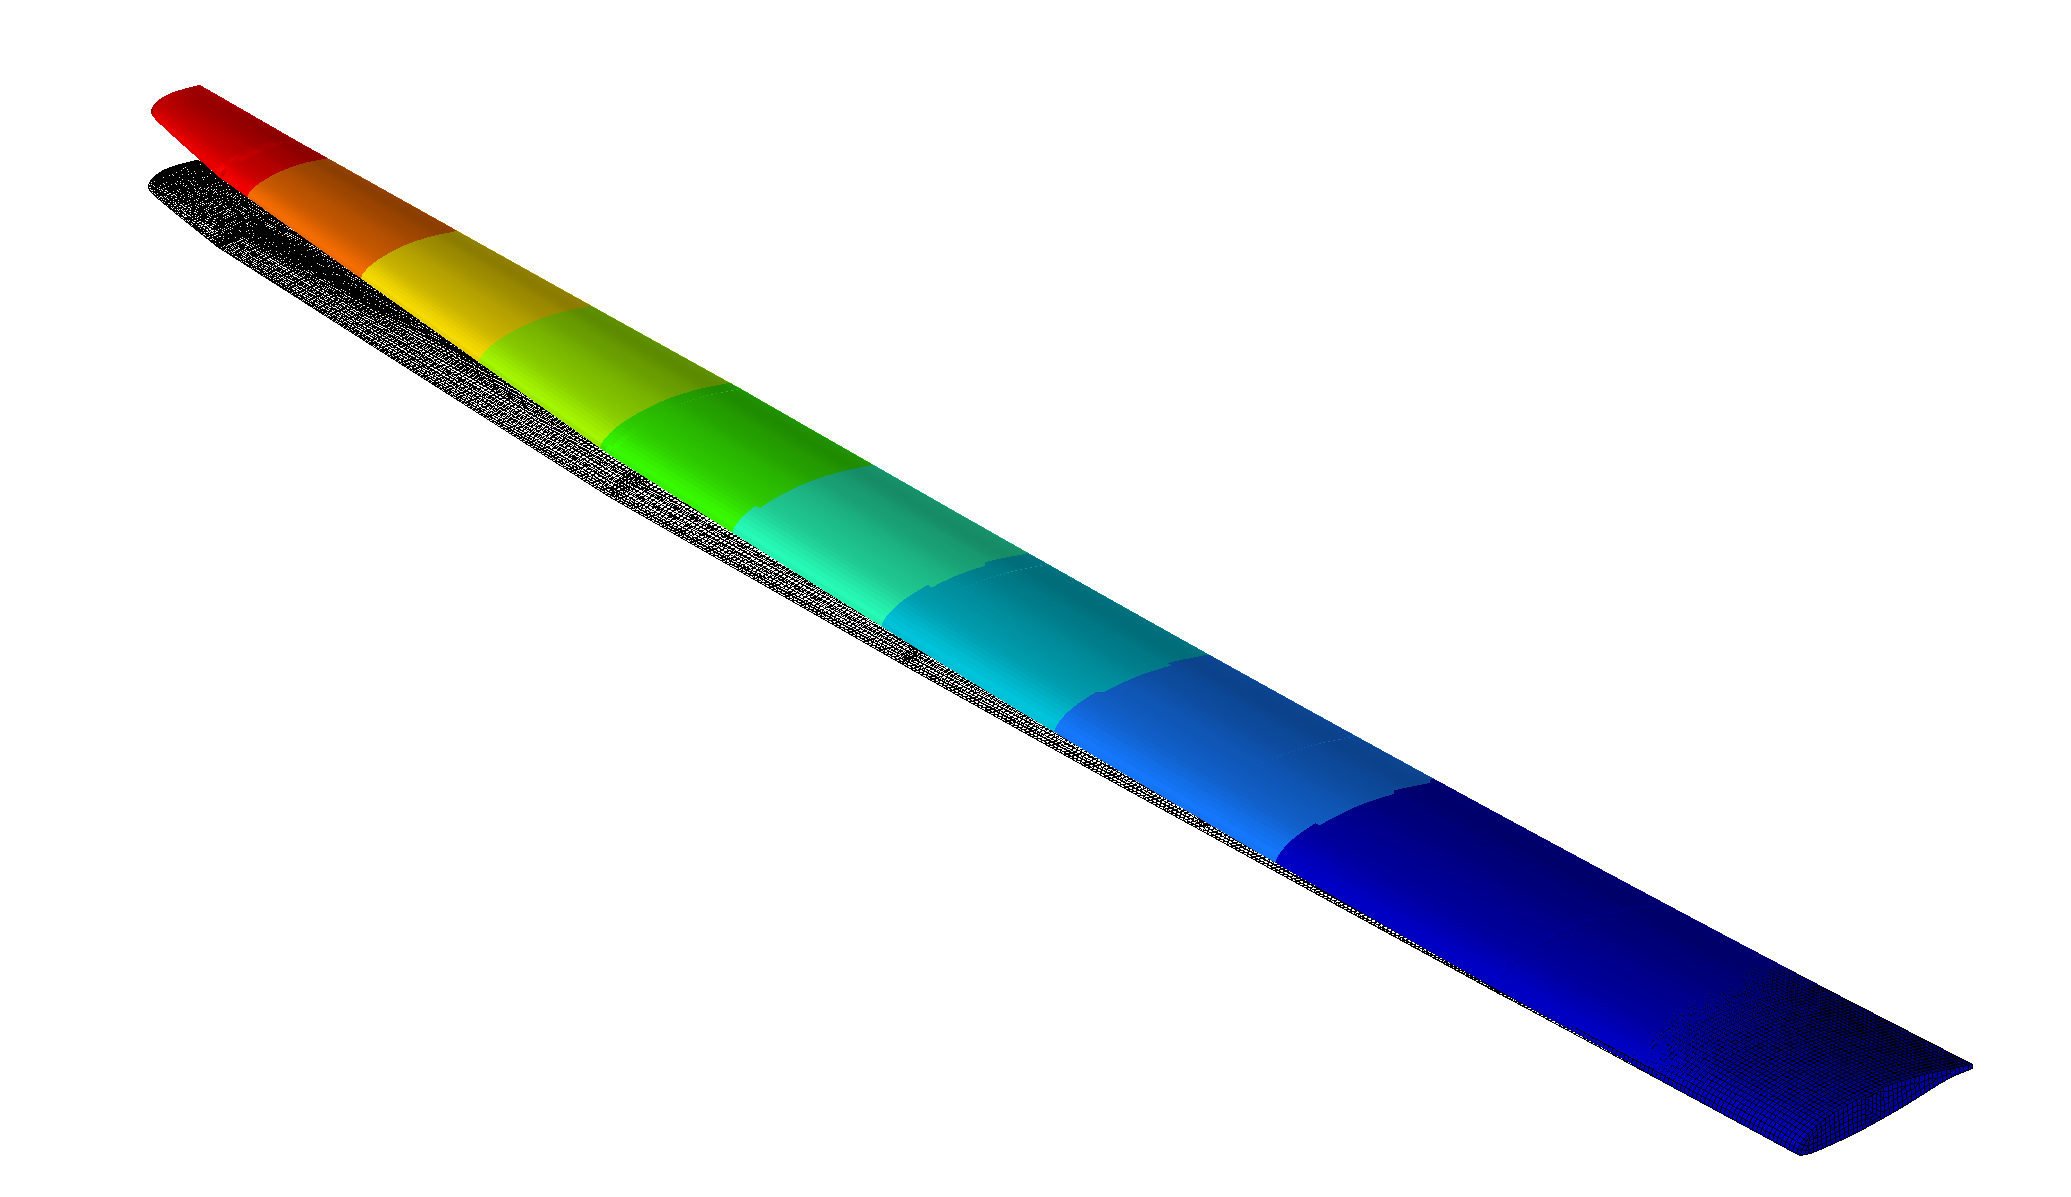
\includegraphics[width=0.5\textwidth]{mode1_1.518Hz.png}}
  \subfloat[Mode 2,\quad $f = 2.704 Hz$]{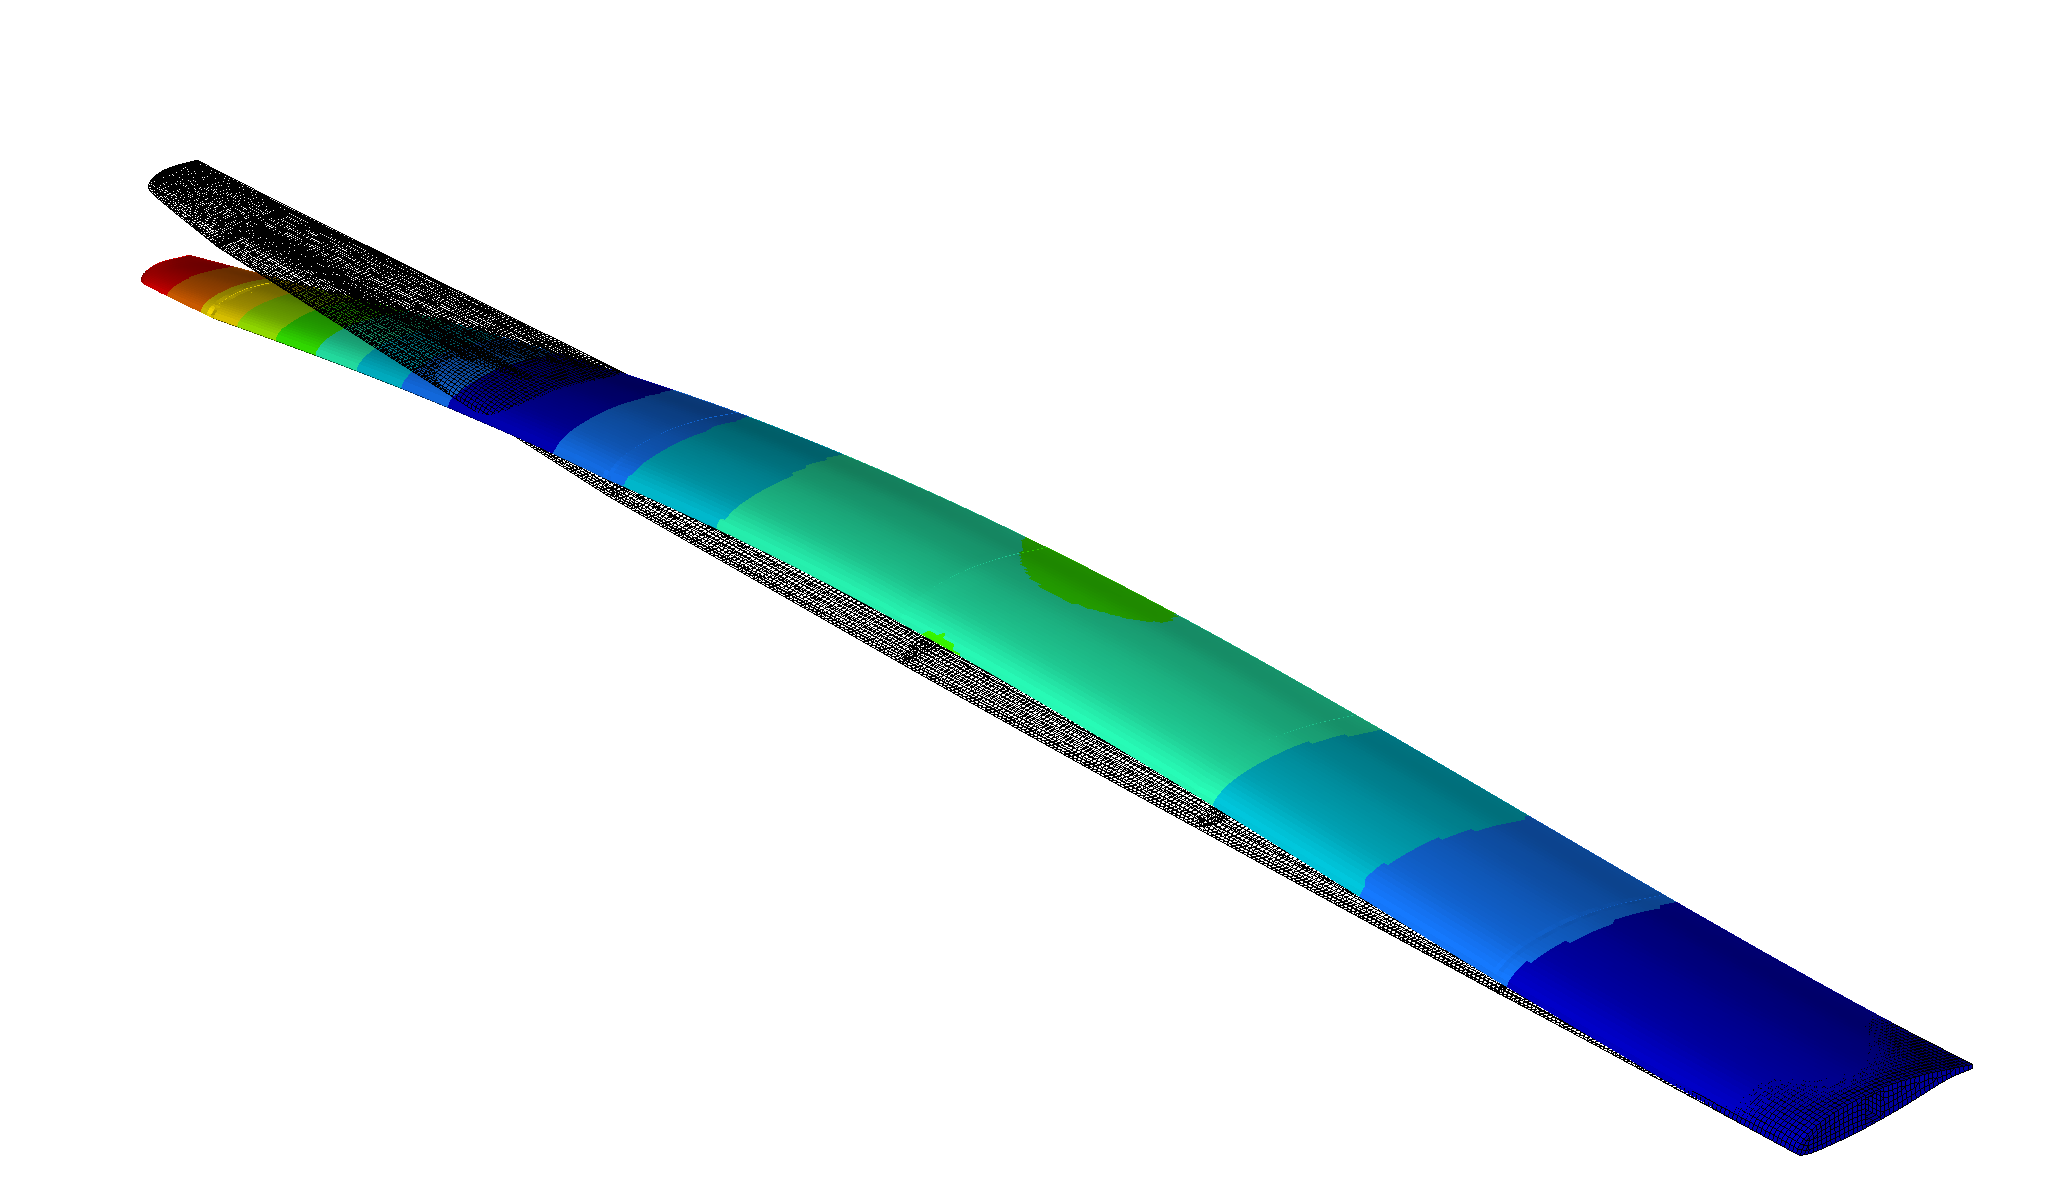
\includegraphics[width=0.5\textwidth]{mode2_7.042Hz.png}}\\
  \subfloat[Mode 3,\quad $f = 7.061 Hz$]{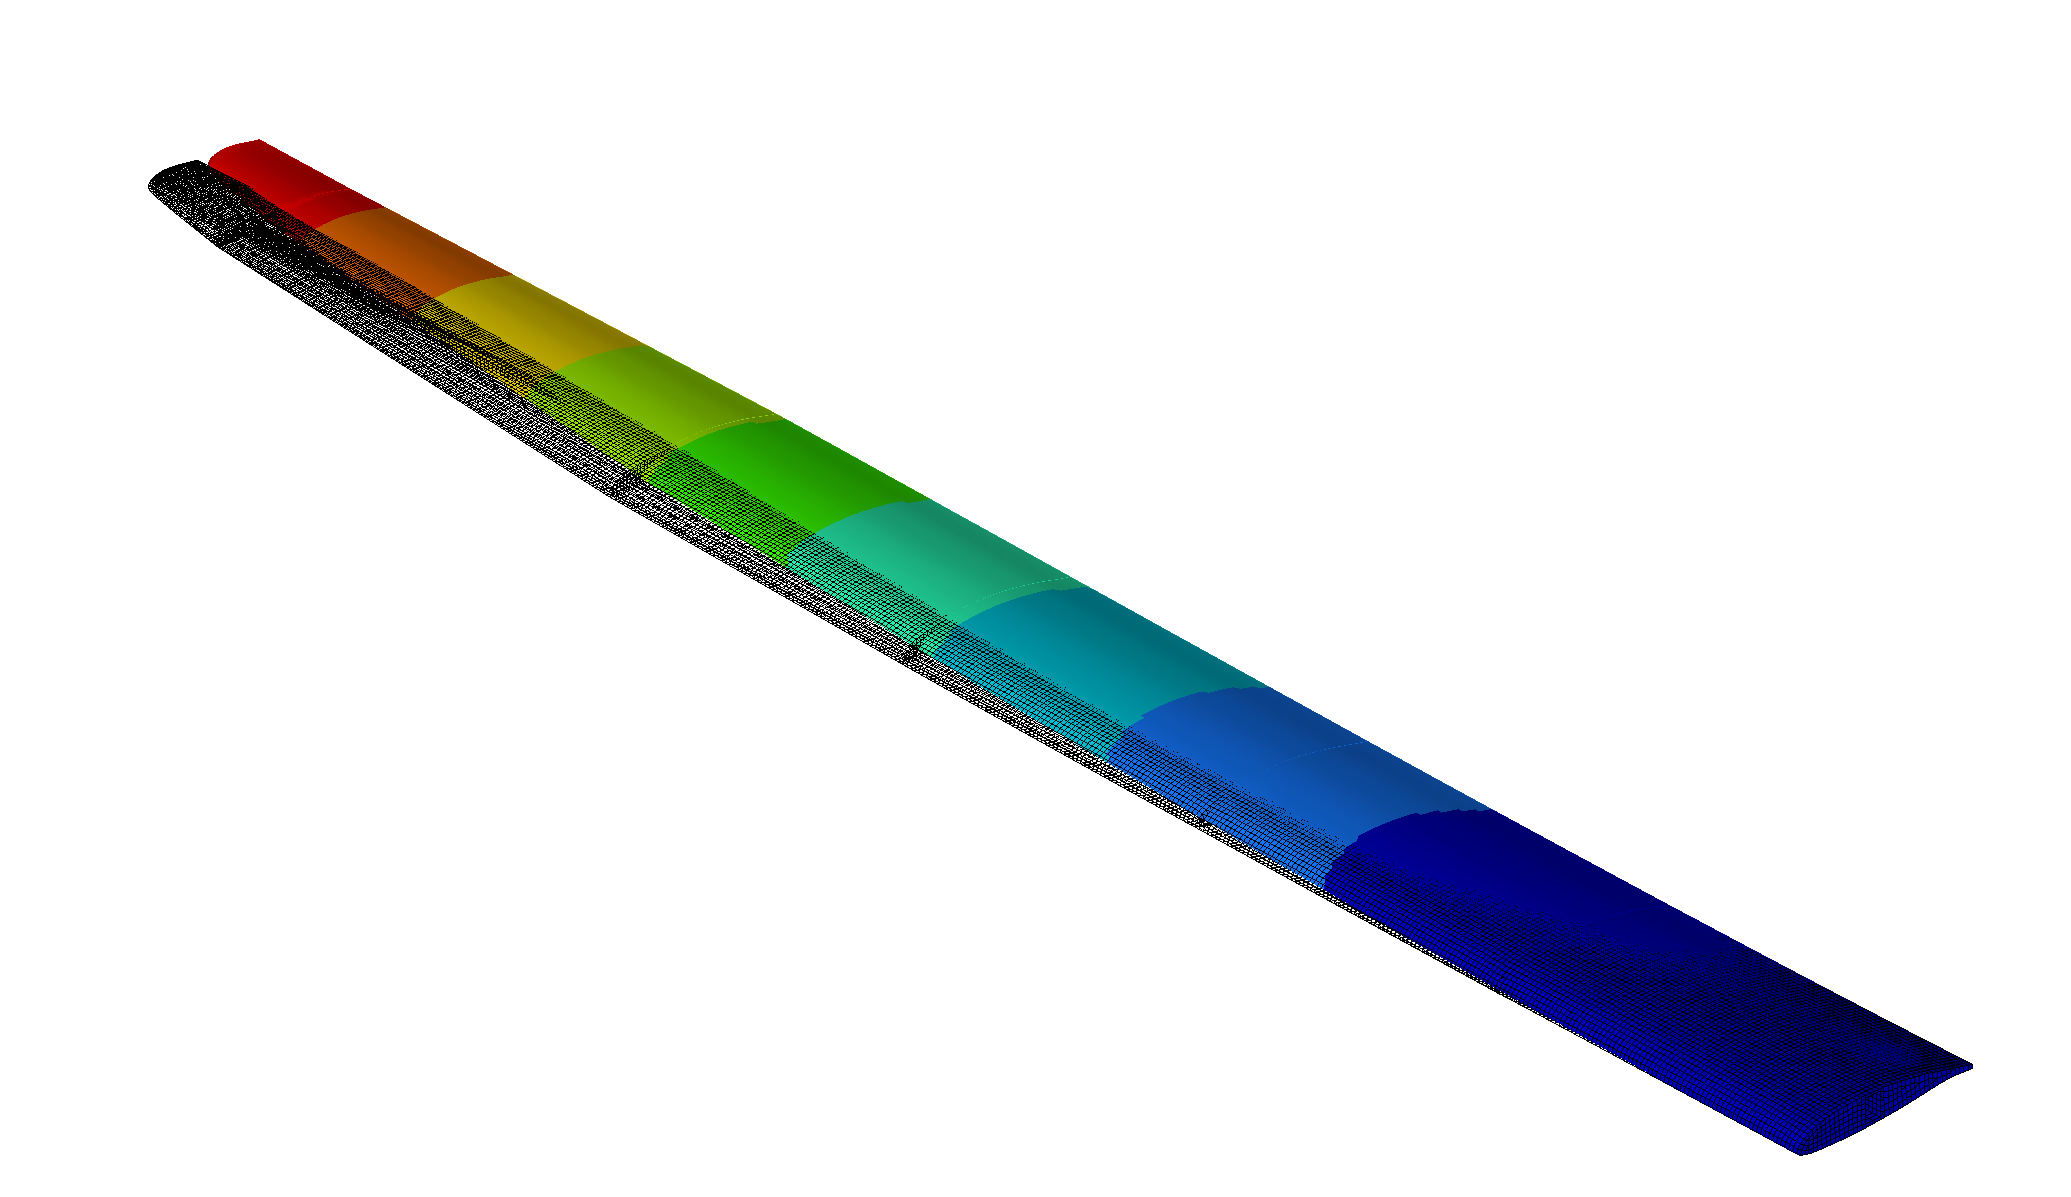
\includegraphics[width=0.5\textwidth]{mode3_7.061Hz.png}} 
  \subfloat[Mode 4,\quad $f = 17.38 Hz$]{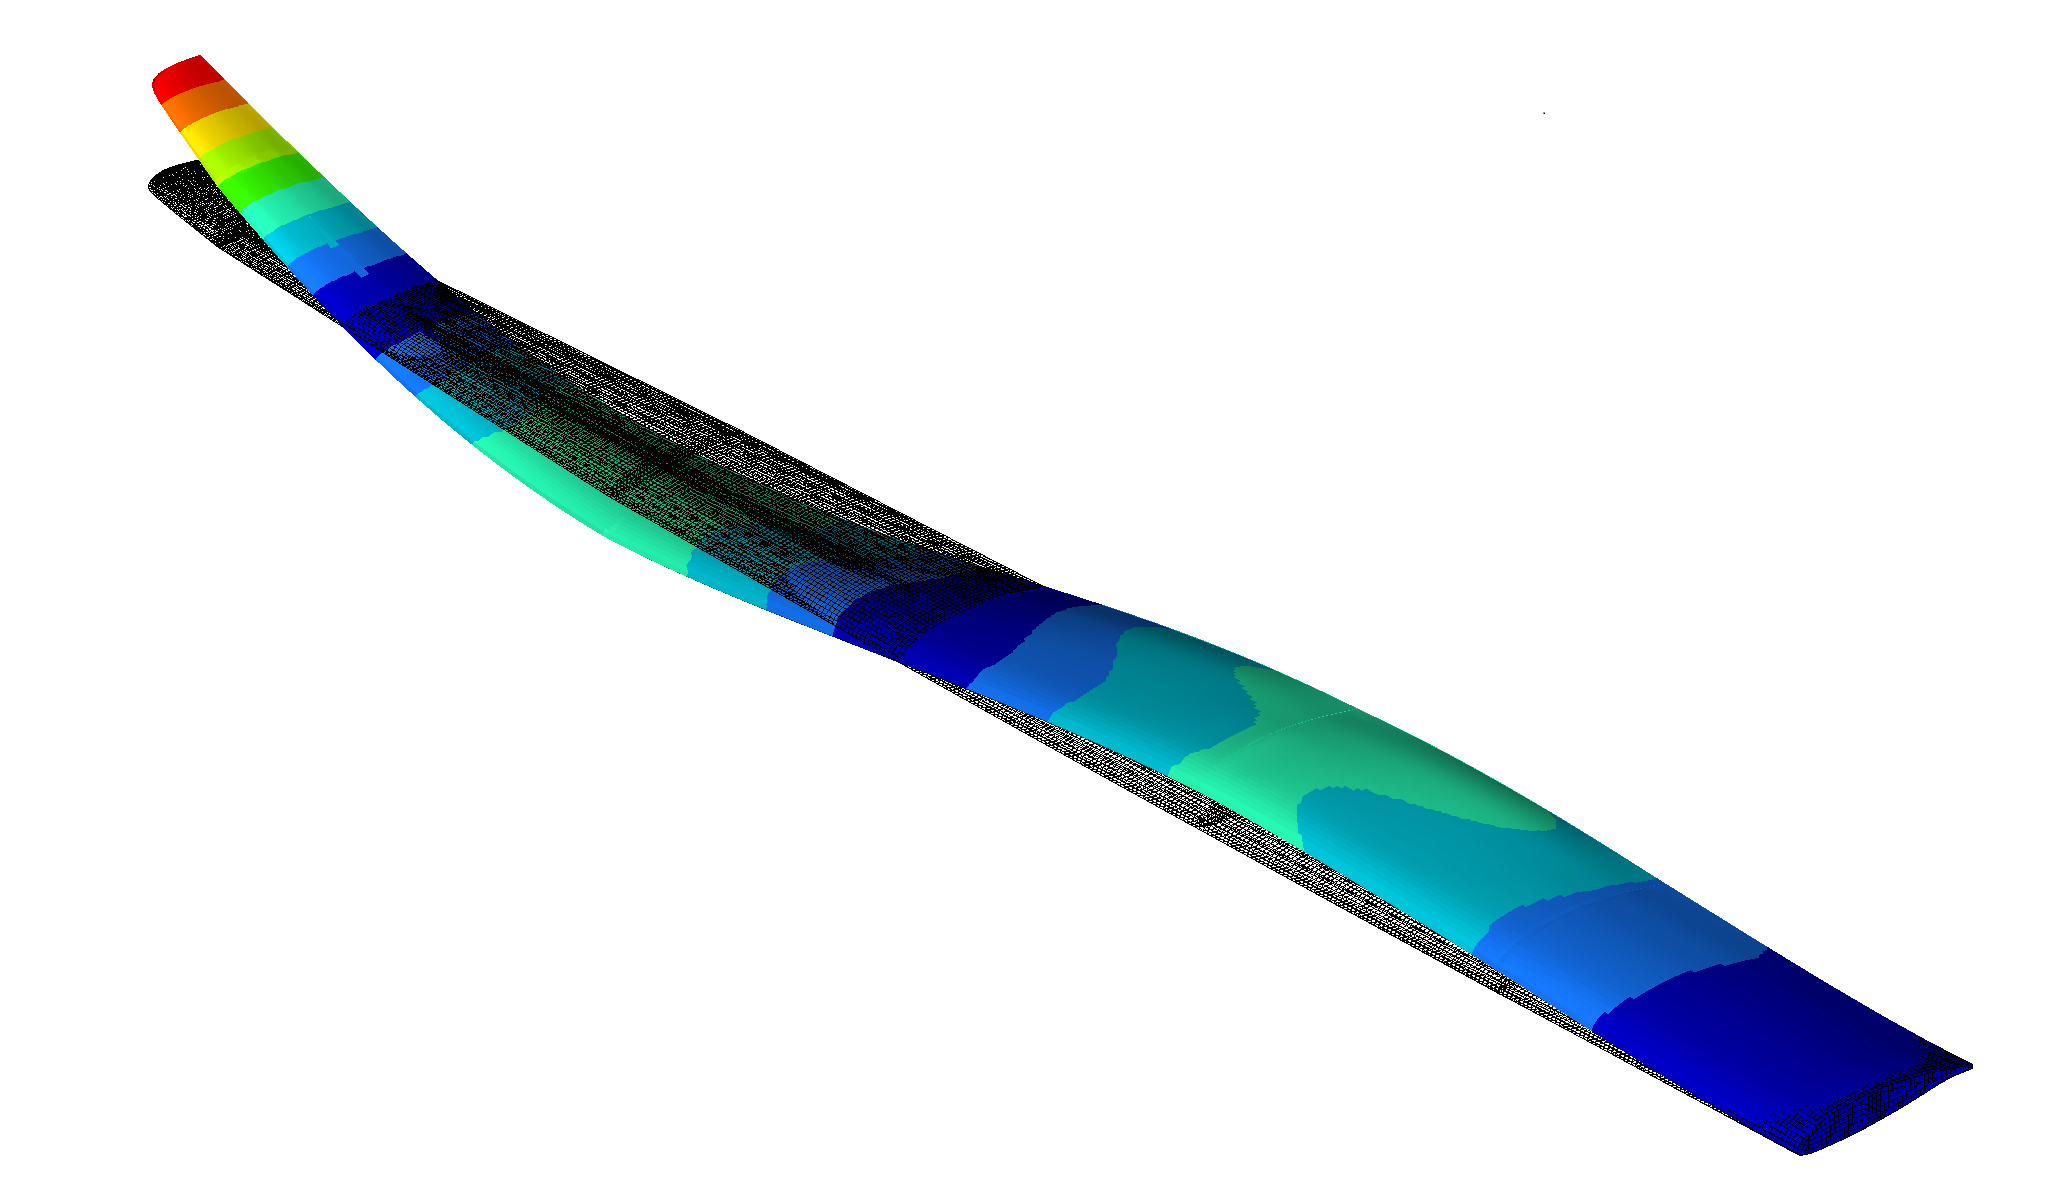
\includegraphics[width=0.5\textwidth]{mode4_17.386Hz.png}}\\
  \subfloat[Mode 5,\quad $f = 30.02 Hz$]{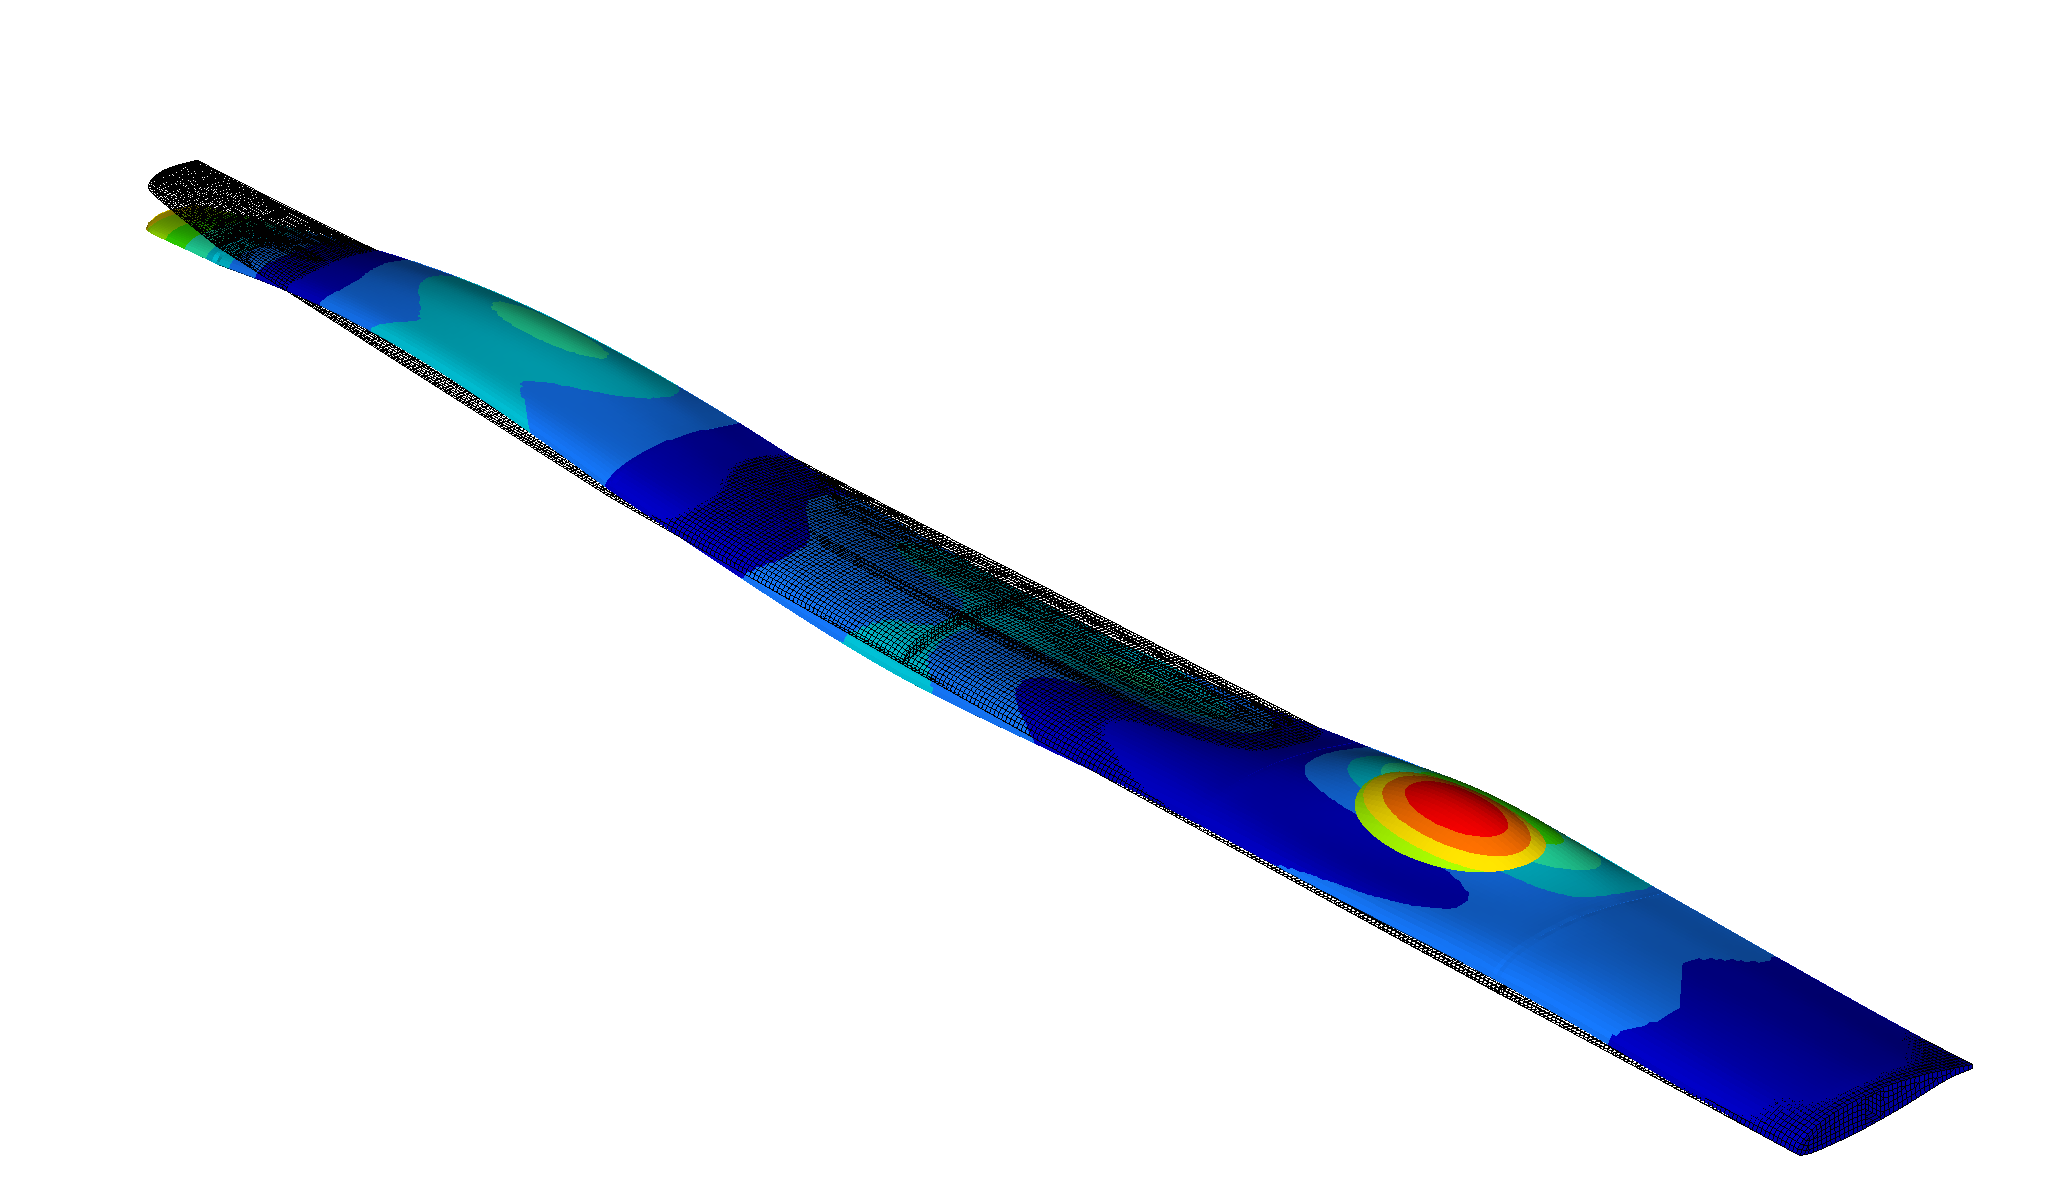
\includegraphics[width=0.5\textwidth]{mode5_30.0168Hz.png}}
  \subfloat[Mode 6,\quad $f = 33.99 Hz$]{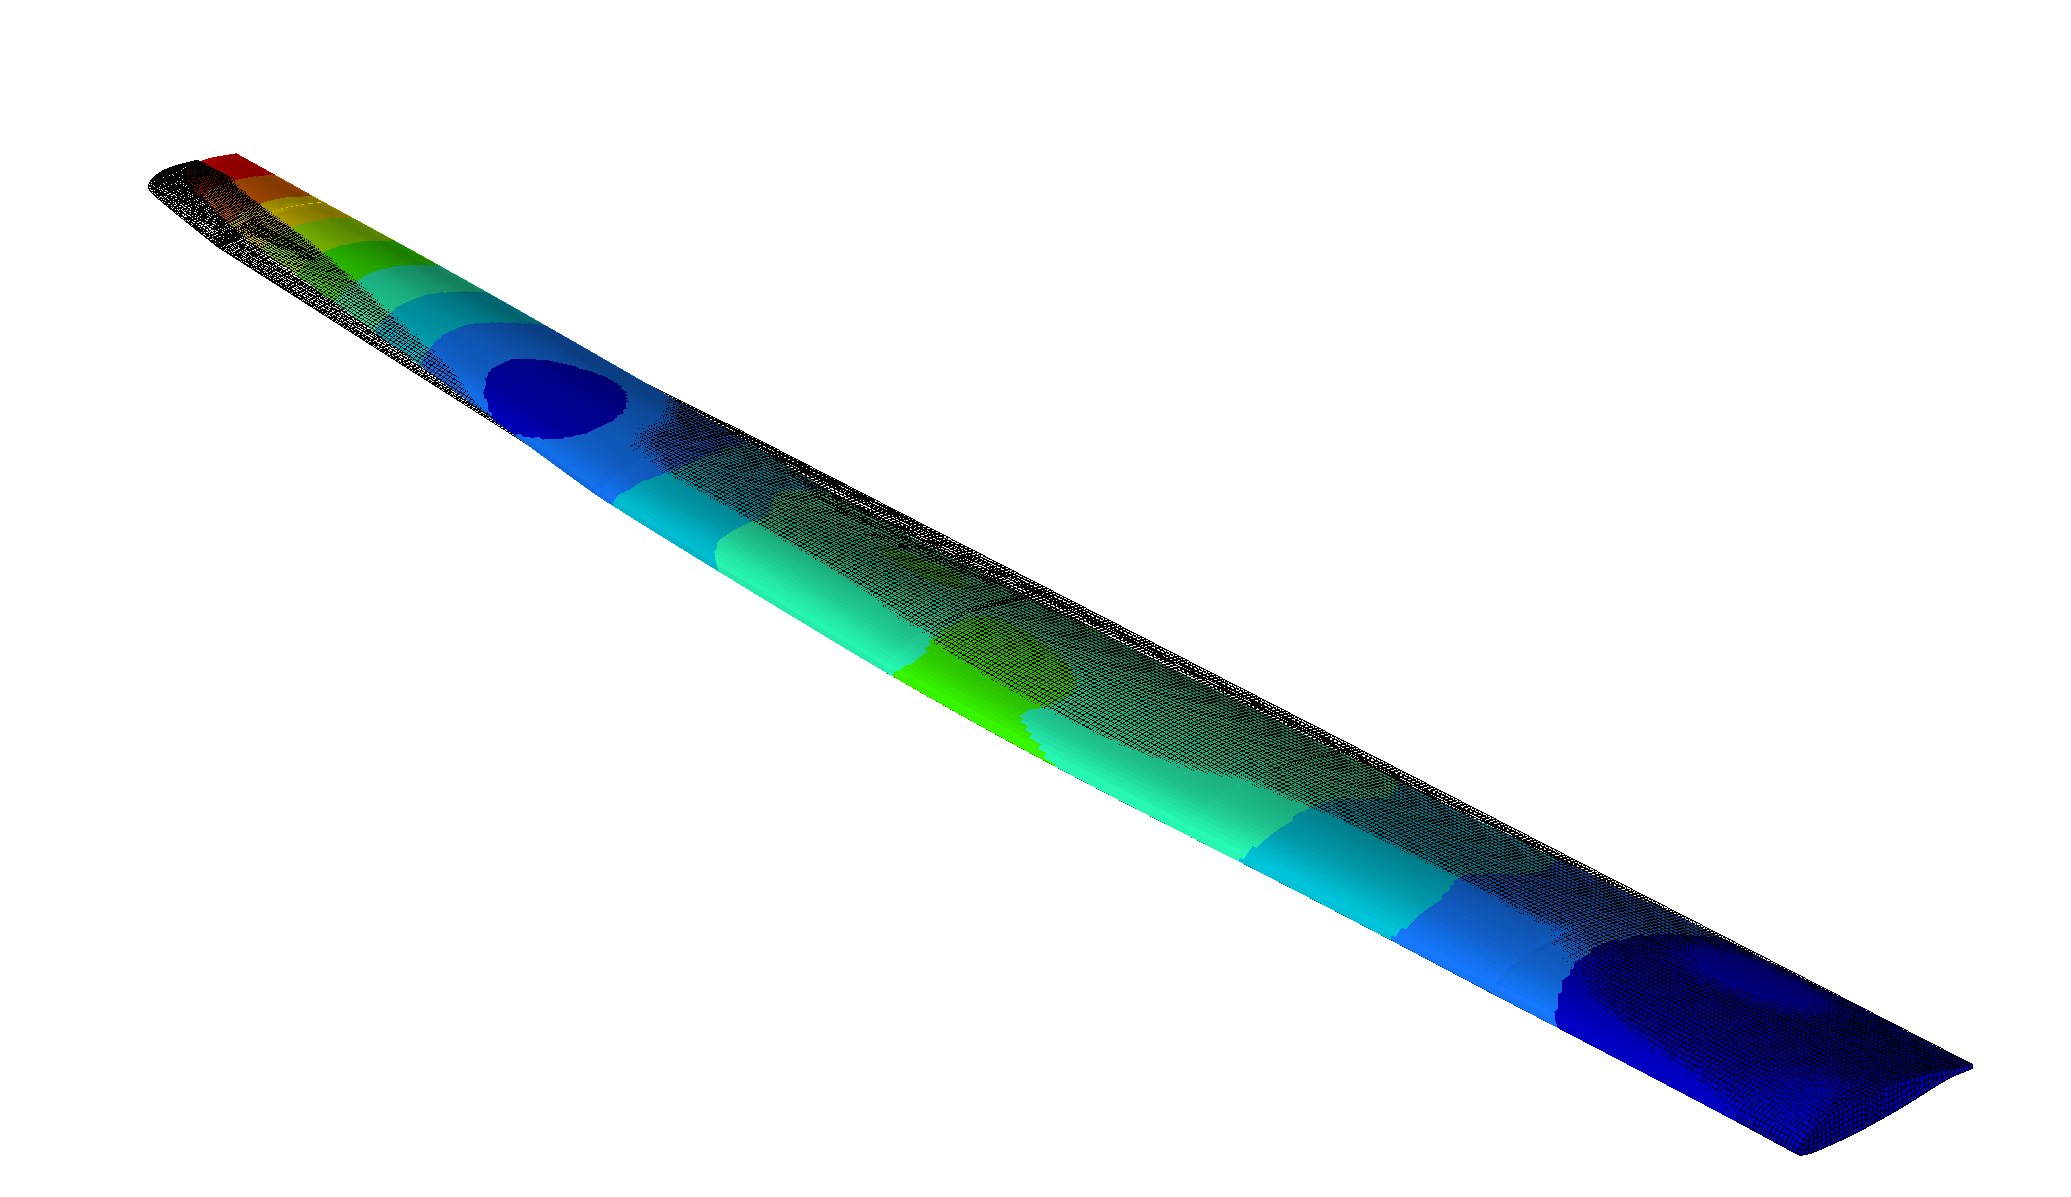
\includegraphics[width=0.5\textwidth]{mode6 33.998Hz.png}}
  \caption{First six Eigenmodes of the ASW 28 Wing}
  \label{fig:asw28modes}
\end{figure}

From \autoref{fig:asw28modes} one can observe the following:

\begin{itemize}
\item
  The first eigenmode has a particularly low frequency indicating that
  the wing is quite flexible in that direction.
\item
  Modes 1, 2, 4 and 5 are all bending modes about the x-axis with an
  increasing number of nodes (stationary points) on the Wing.

  \begin{itemize}
  \item
    Mode 1 is the simplest with just one node at the rooth of the wing.
    As the frequency increases so does the complexity of the bending
    motion and the number of nodes.
  \item
    Mode 2 has two nodes one at the root of the wing and one at about
    three quarters of the wingspan
  \item
    Mode 4 has three nodes one at the root of the wing, one in the
    middle and one approximately 5/6ths of the wingspan
  \item
    Mode 5 has four nodes spread across the wingspan but also exhibits
    some signs of plate vibration on the upper surface of the wing close
    to the root, where the ribs are farthest apart and there exists a
    large section of wing skin which is unsupported.
  \end{itemize}
\item
  Modes 3 and 6 are bending about the z-axis. Mode 3 has only one node
  while mode 6 has two.
\end{itemize}

\section{Initial Flutter Analysis}
\label{initial-flutter-analysis}

By applying the methodology developed in \autoref{asw-28-main-composite-wing-model} to the model the
following results are obtained:

\begin{figure}[H]
    \centering
    \includesvg[width=\textwidth]{initialFlutter.svg}
    \caption{Initial Flutter plot for the first four modes}
    \label{fig:initflutter}
\end{figure}


\begin{figure}[H]
    \centering
    \includesvg[width=\textwidth]{InitialFlutterMode3.svg}
    \caption{Flutter plot of the 3\textsuperscript{rd} mode}
    \label{fig:initfluttermode3}
\end{figure}

From \autoref{fig:initflutter} and \autoref{fig:initfluttermode3} we can see that Flutter occurs on the
3\textsuperscript{rd} mode at:

\begin{equation}
V_{flutter} = 94.11\ m/s
\end{equation}

Notice that Mode 1 is very likely to also diverge at about the same
velocity even though its damping does not change sign. The abrupt
increase of the damping to a value close to zero (but still negative)
along with the reduction of the frequency to almost zero indicate some
form of instability which is not captured by the algorithm since the
sign hasn't technically changed.

\section{Powell's Optimization Method}
\label{powells-optimization-method}

After applying Powell's Optimization method as described in \autoref{applying-powells-method} the following results are obtained

\subsubsection{Scenario 1:}

This was the first objective function which was formulated in equation \eqref{eq:objpowell1} as it defines a more complete optimization problem. The optimization concluded with partial success. The results can be seen in \autoref{fig:ValueofobjectivefunctionthroughouttheoptimizationScenario1}:
\begin{figure}[H]
    \centering
    \includesvg[width=\textwidth]{Objective1.svg}
    \caption{Value of objective function throughout the optimization (Scenario 1)}
    \label{fig:ValueofobjectivefunctionthroughouttheoptimizationScenario1}
\end{figure}

\begin{figure}[H]
    \centering
    \includesvg[width=\textwidth]{Variables1.svg}
    \caption{value of every optimization variable throughout the optimization process (Scenario 1)
    }
\end{figure}

As can be seen the algorithm fails to improve the objective function beyond the initial point. On the first iteration the algorithm tries to reduce the mass of the wing by reducing the thickness of the layers by a tenth of a millimeter, but the flutter speed decreases too much and the penalty is applied resulting in a very high objective function value.

After that point the algorithm experiments with greater values of thickness which of course result in greater mass but sufficiently high flutter speed for the penalty to not apply.

Finally, the algorithm reduces the thickness of the layers incrementally until it reaches the initial thickness.

The algorithm never figures out that by changing the ply angles first so that the flutter speed increases and then reducing the thickness, the flutter speed remains high enough for the penalty to not aplly and the mass is reduced. This is a complicated solution since the angles do not directly affect the mass but only the flutter speed. Had the algorithm explored the angles better while it was in the penalty zone it could have increased the flutter speed sufficiently to get out of the penalty zone and ultimately find a better solution. Unfortunately, this behavior is quite complex and is beyond the capabilities of this relatively simple algorithm.

The Flutter analysis results of the final solution of this algorithm are
shown in \autoref{fig:FlutteranalysisplotsfromPowellsmethodScenario1} and \autoref{fig:Mode3FlutteranalysisPowellsmethodScenario1}:

\begin{figure}[H]
    \centering
    \includesvg[width=\textwidth]{Flutter1.svg}
    \caption{Flutter analysis plots from Powell's method (Scenario 1)}
    \label{fig:FlutteranalysisplotsfromPowellsmethodScenario1}
\end{figure}

The first mode that diverges is mode three which is plotted on its own in the following figure to be able to clearly see when the damping
changes sign.

\begin{figure}[H]
    \centering
    \includesvg[width=\textwidth]{Flutter1Mode3.svg}
    \caption{Mode 3 Flutter analysis Powell's method (Scenario 1)}
    \label{fig:Mode3FlutteranalysisPowellsmethodScenario1}
\end{figure}

The speed at which this mode first diverges is called the flutter speed
and in this case:

\begin{equation}
V_{flutter} = 99.48\ m/s
\end{equation}

\subsubsection{Scenario 2:}

To obtain a better result the simplified objective function from
equation \eqref{eq:objpowell2} is used. This time the algorithm explores the possibility-space with greater success. The results can be seen in \autoref{fig:objpowell2}:

\begin{figure}[H]
    \centering
    \includesvg[width=\textwidth]{Objective2.svg}
    \caption{Value of objective function throughout the optimization (Scenario 2)}
    \label{fig:objpowell2}
\end{figure}

\begin{figure}[H]
  \centering
  \includesvg[width=\textwidth]{Variables2.svg}
  \caption{value of every optimization variable throughout the optimization process (Scenario 2)}
\end{figure}

One can observe from \autoref{fig:objpowell2} that the objective function, which is now the minimization of the negated flutter speed, is significantly improved.

Moreover, as per the definition of this problem the thickness variable remains constant and equal to the initial value of 0.5 mm. This means that while the flutter speed increases significantly the mass remains
constant.

The flutter plots for the optimal solution are now presented for this
method.

\begin{figure}[H]
    \centering
    \includesvg[width=\textwidth]{Flutter2.svg}
    \caption{Flutter analysis plots from Powell's method (Scenario 2)}
\end{figure}


\begin{figure}[H]
    \centering
    \includesvg[width=\textwidth]{Flutter2Mode3.svg}
    \caption{Mode 3 Flutter analysis plots from Powell's method (Scenario 2)}
\end{figure}

Again, the first mode that diverges is mode 3. This time though at a much greater speed than before.

\begin{equation}
V_{flutter} = 175.28\ m/s
\end{equation}

Modes one and four also eventually diverge at $267.09$ and $177.14 m/s$ respectively. As is obvious this is a great improvement of the flutter speed of the wing from the initial solution, without any extra material and thus the same mass as the original wing.

The solution vector that gives the optimum solution is:\\
\begin{equation}
{\vec{\mathbf{x}}}_{opt} = \lbrack 0.0005,90, - 58, - 59\rbrack^{T}
\end{equation}


\section{Genetic Algorithm Optimization}
\label{genetic-algorithm-optimization}

After applying the genetic algorithm as described in chapter 3.4.2 the
following results are obtained:
\begin{figure}[H]
    \centering
    \includesvg[width=\textwidth]{fitness.svg}
    \caption{Evolution of the Fitness metrics of the best solution of every generation in the optimization process}
    \label{fig:fitnessevolution}
\end{figure}


\begin{figure}[H]
    \centering
    \includesvg[width=\textwidth]{genes.svg}
    \caption{Evolution of gene Values throughout the optimization process}
\end{figure}



From \autoref{fig:fitnessevolution} where the best solution found thus far at every generation is plotted, it is observed that both goals are improved by the end of the optimization process, even though those goals are contradictory to one another. From the optimization logs the best solution has the following characteristics.

\begin{equation}
V_{flutter} = 214.69\ m/s,\quad Mass = 45.1\ kg
\end{equation}

The gene values which result in the optimal solution are:

\begin{equation}
t = 0.0003\ mm,\ \ \vartheta_{1} = 43{^\circ},\ \ \vartheta_{2} = 56{^\circ},\ \ \vartheta_{3} = 76{^\circ}
\end{equation}

The flutter plot for this solution is presented in \autoref{fig:FlutterPlotfromGeneticAlgorithm}:
\begin{figure}[H]
    \centering
    \includesvg[width=\textwidth]{FlutterPlot4modes.svg}
    \caption{Flutter Plot from Genetic Algorithm}
    \label{fig:FlutterPlotfromGeneticAlgorithm}
\end{figure}

\begin{figure}[H]
    \centering
    \includesvg[width=\textwidth]{FlutterPlotmode1.svg}
    \caption{Mode 1 Flutter Plot from Genetic Algorithm}
    \label{fig:GAflutterMode1}
\end{figure}

Even though the solution obtained by the genetic algorithm appears ideal,
by examining \autoref{fig:GAflutterMode1} we can see that instability likely occurs earlier than the stated $214 m/s$ as the damping of this mode changes dramatically at $110 m/s$ and the frequency drops to zero which is a sign of flutter. Even if the damping remains negative in this region small changes to the modal characteristics to the wing or even modelling error could lead the real structure to flutter. This is a marginally acceptable solution that would have to be investigated further to ensure its validity

\section{Neural Network Prediction Results}
\label{neural-network-prediction-results}

In this section the results of every Neural Network developed in \autoref{flutter-speed-prediction-using-neural-networks} will be reviewed. Three basic plots are presented to understand
the performance of each network.

\begin{enumerate}
\def\labelenumi{\arabic{enumi}.}
\item
  The first plot, is the value of the loss function on the training and
  validation data at each epoch of training.
\item
  The second plot, is used to judge the performance of the network by
  plotting the \(y_{pred}\ vs\ y_{true}\) scatter plot. Ideally these
  values would match thus producing a straight line at a \(45{^\circ}\)
  angle.
\item
  The third plot, plots the residuals with respect to y true
  \( (y_{\text{true}} - y_{\text{pred}}) \text{ vs } y_{\text{true}} \) which makes it easier to
  understand the magnitude of the error as well as any trends that might
  exist at particular flutter speeds.
\end{enumerate}

\subsection{Training data examination}
\label{training-data-examination}

A preliminary exploration of the data is done using a pair plot, which is a matrix of graphs the enables the visualization of the relationship between each pair of variables in the dataset.

\begin{figure}[H]
    \centering
    \includesvg[width=\textwidth]{DataExploration/pairplot.svg}
    \caption{Pair Plot of training data}
    \label{fig:pairplot}
\end{figure}

From \autoref{fig:pairplot} we can observe the following relationships in the gathered data:

\begin{enumerate}
\def\labelenumi{\arabic{enumi}.}
\item
  As thickness increases so does the predicted flutter speed.
\item
  The angles \(\theta_{1} - \theta_{3}\) have a strongly nonlinear
  correlation with flutter speed with no obvious trends
\item
  Along the diagonal histograms which represent the correlation of a
  variable with itself it can be observed that the data is randomly and
  evenly distributed across the range of possible values.
\end{enumerate}

\subsection{1 Hidden Layer Neural Network}\label{hidden-layer-neural-network}

\begin{figure}[H]
  \centering
  \subfloat[training history]{\includesvg[width=0.5\textwidth]{1HL/traininghistory.svg}} \\
  \subfloat[$Y_{true}$ vs $Y_{pred}$]{\includesvg[width=0.5\textwidth]{1HL/Ytrue_vs_Ypred.svg}}
  \subfloat[Residulas]{\includesvg[width=0.5\textwidth]{1HL/Residuals_vs_Ytrue.svg}}

  \caption{1 Hidden Layer Neural Network Performance}
  \label{fig:1HLNNperf}
\end{figure}

From \autoref{fig:1HLNNperf} it becomes apparent that even though this model with only one hidden layer was given 400 epochs to train, which is a lot, as will become evident by the following results, the validation data Mean Average Error is too great for the network to be of any use. The variance above and below the zero line in \autoref{fig:1HLNNperf} $c$ is way too great with many points being over or underestimated by more
than $50 m/s$

\subsection{2 Hidden Layer Neural Network}
\label{hidden-layer-neural-network-1}
\begin{figure}[H]
  \centering
  \subfloat[training history]{\includesvg[width=0.5\textwidth]{2HL/traininghistory.svg}} \\
  \subfloat[$Y_{true}$ vs $Y_{pred}$]{\includesvg[width=0.5\textwidth]{2HL/Ytrue_vs_Ypred.svg}}
  \subfloat[Residulas]{\includesvg[width=0.5\textwidth]{2HL/Residuals_vs_Ytrue.svg}}

  \caption{2 Hidden Layer Neural Network Performance}
  \label{fig:2HLNNperf}
\end{figure}

This model was trained for 350 epochs. 2 Hidden layers perform much better than a single layer. The mean average error on the validation data by the end of the training is about $7 m/s$. The only problem is that there is still great variance in the predictions as can be seen from \autoref{fig:2HLNNperf}.

\subsection{4 Hidden Layer Neural Network}
\label{hidden-layer-neural-network-2}

\begin{figure}[H]
  \centering
  \subfloat[training history]{\includesvg[width=0.5\textwidth]{4HL/traininghistory.svg}} \\
  \subfloat[$Y_{true}$ vs $Y_{pred}$]{\includesvg[width=0.5\textwidth]{4HL/Ytrue_vs_Ypred.svg}}
  \subfloat[Residulas]{\includesvg[width=0.5\textwidth]{4HL/Residuals_vs_Ytrue.svg}}

  \caption{4 Hidden Layer Neural Network Performance}
  \label{fig:4HLNNperf}
\end{figure}

The four hidden layer neural network was trained for 300 epochs because the validation loss starts to flatten out as can be seen from \autoref{fig:4HLNNperf}. The spread of data around the zero residual line is not much tighter than the previous model.

\subsection{6 Hidden Layer Neural Network}
\label{hidden-layer-neural-network-3}

\begin{figure}[H]
  \centering
  \subfloat[training history]{\includesvg[width=0.5\textwidth]{6HL/traininghistory.svg}} \\
  \subfloat[$Y_{true}$ vs $Y_{pred}$]{\includesvg[width=0.5\textwidth]{6HL/Ytrue_vs_Ypred.svg}}
  \subfloat[Residulas]{\includesvg[width=0.5\textwidth]{6HL/Residuals_vs_Ytrue.svg}}

  \caption{6 Hidden Layer Neural Network Performance}
  \label{fig:6HLNNperf}
\end{figure}
The 6 Hidden layer neural network was trained for 250 epochs to prevent overfitting as the validation loss is stagnant after epoch 220. This can be seen in \autoref{fig:6HLNNperf}

The spread of the residuals is better but still high but getting better in relation to the previous model as can be seen in Figure \autoref{fig:6HLNNperf} $c$.

\subsection{Hyperparameter tuned Neural Network}
\label{hyperparameter-tuned-neural-network}

The hyperparameters that were chosen from the HyperBand algorithm which was described in \autoref{flutter-speed-prediction-using-neural-networks} are as follows:

\begin{itemize}
\item
  Number of hidden layers: 5
\item
  Number of Neurons for each layer:
  \(1024,\ \ 512,\ \ 256,\ \ 512,\ and\ 1024\) respectively
\item
  Activation function for every layer: ReLu
\item
  Learning Rate of Adam Optimizer: 0.001
\end{itemize}

The Resulting structure of the model can be seen in \autoref{fig:HypertunedStructure}.

\begin{figure}
  \centering
  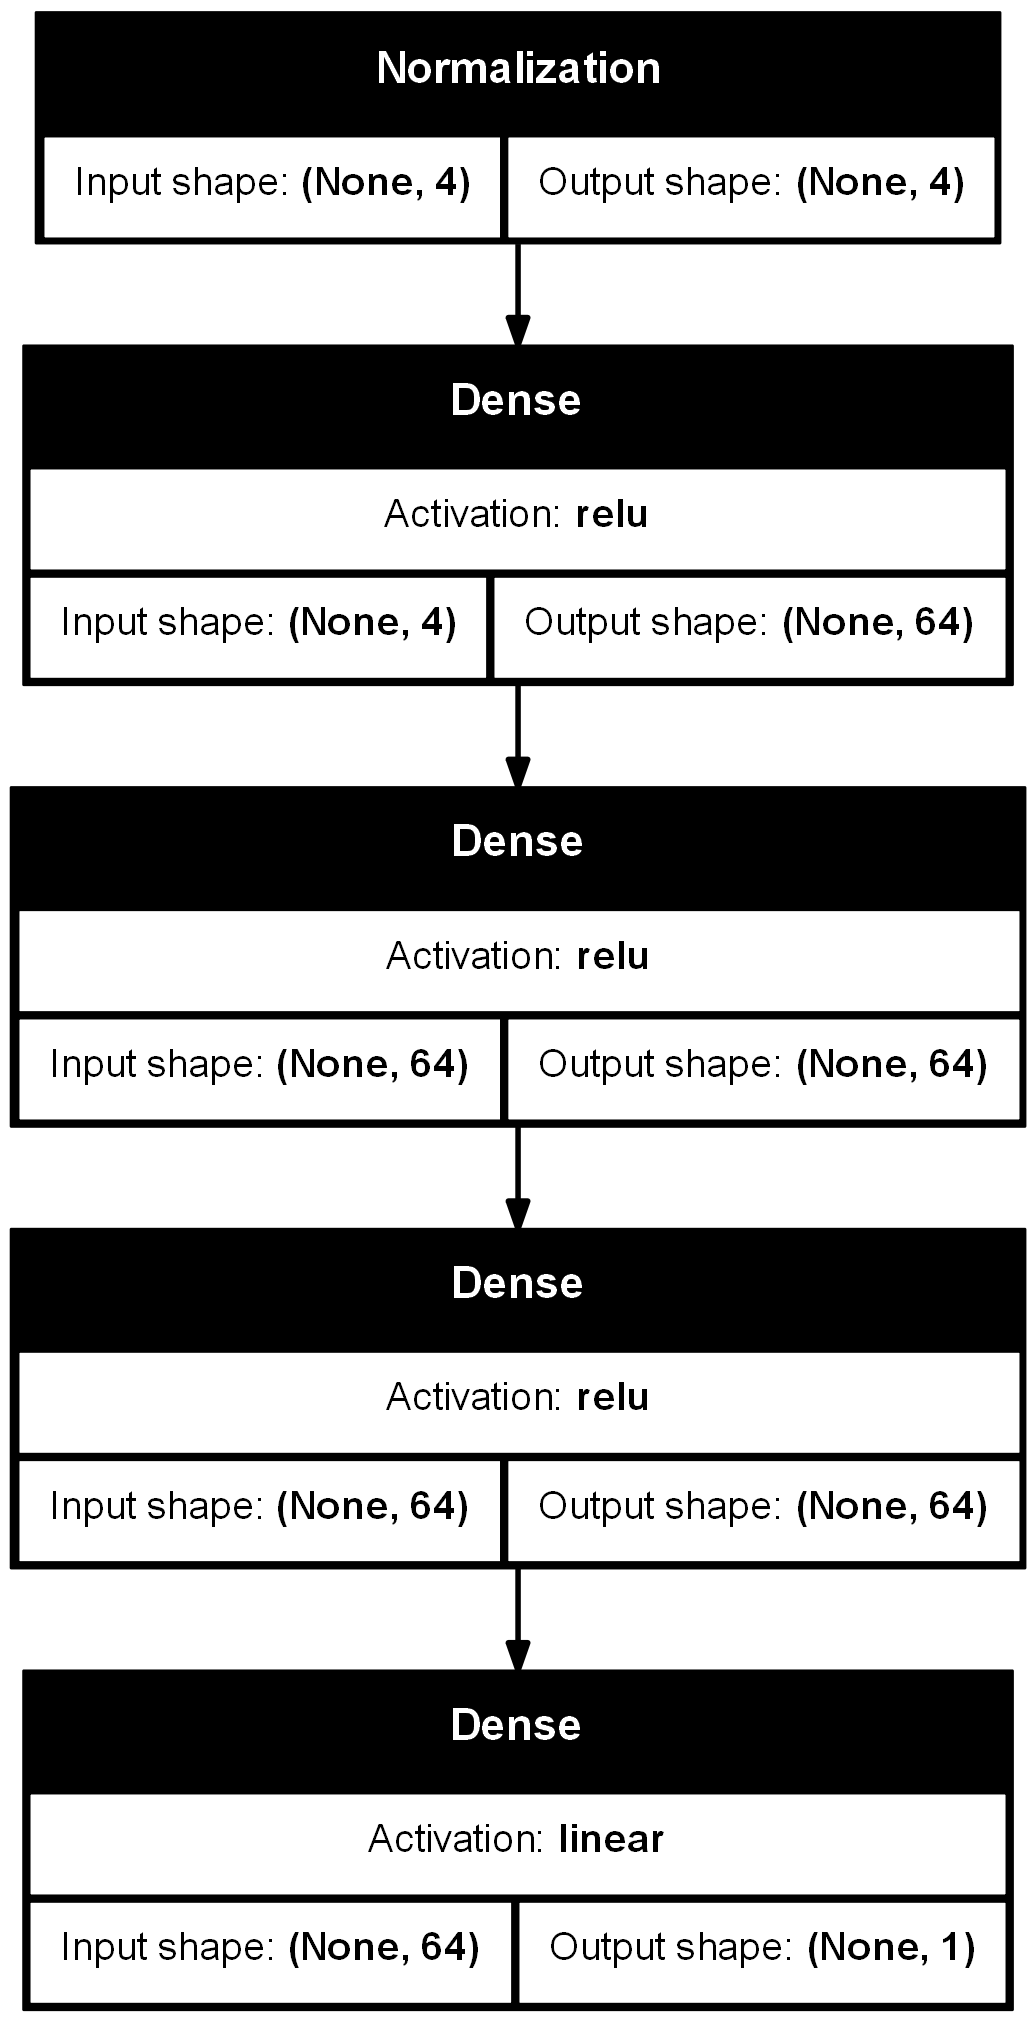
\includegraphics[width=0.38\textwidth]{tunedmodel_24_09_2024/structure.png} 
  \caption{Hypertuned model structure.}
  \label{fig:HypertunedStructure}
\end{figure}

\begin{figure}[H]
  \centering
  \subfloat[training history]{\includesvg[width=0.5\textwidth]{tunedmodel_24_09_2024/traininghistory.svg}} \\
  \subfloat[$Y_{true}$ vs $Y_{pred}$]{\includesvg[width=0.5\textwidth]{tunedmodel_24_09_2024/Ytrue_vs_Ypred.svg}}
  \subfloat[Residulas]{\includesvg[width=0.5\textwidth]{tunedmodel_24_09_2024/Residuals_vs_Ytrue.svg}}

  \caption{Hypertuned Neural Network Performance}
  \label{fig:HypertunedNNperf}
\end{figure}

As can be seen from \autoref{fig:HypertunedNNperf} this model was trained for 200 epochs
because the validation MAE stops decreasing after that. This model
exhibits the lowest MAE of every other model with a validation
\(MAE < 5 m/s\).

What is more, the distribution of data around the Zero Residual Line in
\autoref{fig:HypertunedNNperf} $c$, is the tightest of all the models thus producing the best
results yet. It is also worth mentioning that this model has the highest
number of trainable parameters and takes the longest to train.
